%% %%%%%%%%%%%%%%%%%%%%%%%%%%%%%%%%%%%%%%%%%%%%%%%%
%% Problem Set/Assignment Template to be used by the
%% Food and Resource Economics Department - IFAS
%% University of Florida's graduates.
%% %%%%%%%%%%%%%%%%%%%%%%%%%%%%%%%%%%%%%%%%%%%%%%%%
%% Version 1.0 - November 2019
%% %%%%%%%%%%%%%%%%%%%%%%%%%%%%%%%%%%%%%%%%%%%%%%%%
%% Ariel Soto-Caro
%%  - asotocaro@ufl.edu
%%  - arielsotocaro@gmail.com
%% %%%%%%%%%%%%%%%%%%%%%%%%%%%%%%%%%%%%%%%%%%%%%%%%

\documentclass[12pt]{article}
\usepackage{design_ASC}
\usepackage{graphicx} %package to manage images
\usepackage{hyperref}

\graphicspath{ {./images/} }

\usepackage[rightcaption]{sidecap}

\usepackage{wrapfig}
\usepackage[english]{babel}
\usepackage{xcolor}
\usepackage{amsmath}
\usepackage{sidecap}  %required for side captions
\usepackage{listings}
\usepackage{xcolor}

\setlength{\parindent}{4em}
\setlength{\parskip}{1em}

\setlength\parindent{0pt} %% Do not touch this
\urlstyle{same}
\hypersetup{
    colorlinks,
    linkcolor={black!50!red},
    citecolor={black!50!blue},
    urlcolor={black!80!blue}
}

%% -----------------------------
%% TITLE
%% -----------------------------
\title{Project 1 \\
Automatic grading of multiple choice tests} %% Assignment Title

\author{Lupașcu Marian\\ %% Student name
Computer Vision\\ %% Code and course name
\textsc{University of Bucharest}
}

\date{\today} %% Change "\today" by another date manually
%% -----------------------------
%% -----------------------------

%% %%%%%%%%%%%%%%%%%%%%%%%%%
\begin{document}
\setlength{\droptitle}{-5em}    

%% %%%%%%%%%%%%%%%%%%%%%%%%%
\maketitle

% --------------------------
% Start here
% --------------------------


% %%%%%%%%%%%%%%%%%%%
\section*{Scenario 1 (real world)}
% %%%%%%%%%%%%%%%%%%%

\emph{You receive a test set containing 55 scanned images annotated with the option (F or I) 
and with the digit (1, 2, 3 or 4). For each image you have to output the corresponding grade.}

This task is reduced to identifying the lines and columns in the two tables filled with answers (Xs)
on both the left and right sides. For line identification, the find\_rows (grayscale\_image) 
function, which receives a grayscale image of a patch in the image, which contains one of two 
tables (either blood or right), filters the image with a Sobel filter of y direction. Following 
this filtering, adding the binarized image and ready on the y axis gives high values ​​in the way 
where there are lines. Eliminating the redundant and land lines the last 16 lines get the desired 
rows, it hurts at the top we have the header of the table that we are not interested in. Of course, 
the parts that do not contain useful information for this task are removed from the image, ie the 
writing below and the header, including the variant and the option. The function 
find\_columns (grayscale\_image) does the same thing fixed in the x direction, obtaining the desired columns.
\par

\includegraphics[scale=0.7]{descărcare2.png}

The function find\_table (grayscale\_image) calls the two functions described above and then cuts the image 
in the first row, the last row the first column and the last column, resulting in the area of ​​interest 
(the one with Xs). Here the most interesting function is find\_x (grayscale\_image, vertical\_lines, 
horizontal\_lines) iterates along the lines and calculates the average of the pixels in the patch 
delimited by vertical\_lines (ie 4 means, A, B, C, D) and then selects in response for the respective 
row (ie the number in the subject) the patch index with the smallest value (the one with the most 
black => has X).
\par

The predict grade scenario 1 (path, subject, number) function loads the image from the path, eliminates 
the redundant parts, cuts it in two, determines the delimiting lines and columns on each side, then 
identifies the student's Xs on both the left and right with find\_x function. Next, knowing the subject 
and the number, I load the correct answers (the scale) and then begin to compare the answers with the 
answers (A, B, C, or D). \textbf{For this task, the accuracy of the 150 images is 100\%.}

% %%%%%%%%%%%%%%%%%%%
\section*{Scenario 2 (intermediate)}
% %%%%%%%%%%%%%%%%%%%

\emph{You receive a test set containing 50 rotated and 50 perspective images annotated with the view 
(rotated or perspective), the option (F or I) and the digit (1, 2, 3 or 4). For each image you have 
to output the corresponding grade.}

Scenario 2 can be reduced very elegantly to Scenario 1 using a hemography matrix that reduces an 
image with a subject in perspective or rotation to a desired template. For this function 
transform\_rotaded\_and\_perspective\_in\_scanned (img\_path, template\_path) transforms the image 
from img\_path into one that looks like a template from template\_path. Initially identify 15000 
keypoints with ORB from both the template and the desired image. 
Then the matches are identified in the two-way between keypoints, 
the first 50\% of these matches are selected, referring to the Hamming distance. 
Finally, the hemography matrix is ​​identified and the image reduced to the template. 
\par

Next a principle identical to Scenario 1 is hypothetically correct. But as an optimization, 
because the warp image (reduced to the template has noise compared to the template) identifies 
the lines and columns on the template (no noise and stable) to be used on the image reduced to 
the template (with noise and more). stable). In the absence of these optimizations \textbf{the accuracy 
for this scenario} is about 90\% and at present it \textbf{is 100\%.} I mention that for perspective, 
rotated or scanned this principle is used.

% %%%%%%%%%%%%%%%%%%%
\section*{Scenario 3 (no annotations)}
% %%%%%%%%%%%%%%%%%%%

\emph{You receive a test set containing 75 images (scanned, rotated or perspective view). There is 
no annotation available. For each image you have to output the corresponding grade.}

For this scenario we will use the detect\_subject\_choice (choice\_patch\_grayscale, rows, cols) 
function that identifies the Informatica and Physics boxes in an image knowing the lines and 
columns (the edges are known to be above the first line and between the last two columns of 
the right-hand side) . Being in this Scenario we do not know neither the subject nor the number 
of the subject we will need some additional tools. To identify the subject is simple: with the 
function of earlier, the boxes are identified then the boxes are sorted by the y coordinate 
and if box 1 has an average of pixels larger than box 2 then it is Informatica otherwise Physics. 
\par

\includegraphics[scale=0.7]{Capturăoo.PNG}

To identify the number is a little trickier. We will need the eval\_patch (patch) function and 
a model (a convolutional network trained on MNIST). The convolutional network trained on the 
MNIST is described in the picture above, and receives as input images of size $28\times28$. We have 
variables ranging from 80 to 100 on 80-100. For preprocessing we have: GaussianBlur with 
$7\times7$ filter for noise elimination, adaptiveThreshold to binarize the image, bitwise\_not to 
deny it (in MNIST is white figure on black background), then cut 5 pixels from all edges 
(corresponding to the figure box) then add 10 pixels on each edge (because in MNISt the 
figures have little edge) finally resize the image to $28\times28$ and pass it to the network. 
\par

Only output indexes 1, 2, 3 and 4 (possible variants in us) are kept from the output activations. 
At this time the accuracy on labels 2 and 3 is 100\%, for 4 of 96\% and for 1 of 50\% 
(confusing only with label 4), because the number 1 from us differs considerably from 
the number 1 from the MNIST. But you can see something if you inspect activations on 
labels 1 and 4 you can set a threshold between these activations:
\begin{lstlisting}[language=Python]
    if pred == 4 and output [3] - output [0] < 2000:
        pred = 1
\end{lstlisting}
achieving a final accuracy of 98\%. The only mistakes are made in the pictures below.
At this moment we have calculated the subject and the number so this Scenario is equivalent 
to Scenario 2, the reduction being a trivial one.
\textbf{Accuracy in this scenario is 95\%.}

\includegraphics[scale=0.6]{descărcare44.png}
The first image is cataloged as 2, the middle one as 3 and the last one as 1.

% %%%%%%%%%%%%%%%%%%%
\section*{Scenario 4 (handwritten recognition)}
% %%%%%%%%%%%%%%%%%%%

\emph{Your receive a test set containing 25 scanned images. We will make sure to modify 
some content such that the grade written in red to be different that the grade obtained 
by a perfect grading system. For each image you have to output the corresponding handwritten grade.}

This scenario is the most difficult because it involves locating the figures in the image. 
Next, the approach involves a series of steps: identifying the global area (with lots of 
backround noise) in which the handwritten notes are located.
\begin{lstlisting}[language=Python]
    image = image[int(orig_h * 0.29):int(orig_h * 0.33)]
    image = image[:, int(orig_w * 0.08):int(orig_w * 0.29)]
\end{lstlisting}
Then transform the image into grayscale, filter the image with a Gaussian Blurr filter of 
size $11\times11$, binarize and finally deny it to be similar to the MNIST format. Then with a 
series of templates the image is cut in different areas (at the first open round bracket and 
at ... from the bottom area). It then removes the background from all areas with the 
cut\_background (image, proj) function (which from the image received as a column parameter 
until it no longer finds columns that are sufficiently black (max. 5 white pixels) that are 
grouped in batches of 10 columns minimum).
\begin{lstlisting}[language=Python]
    new_th = cut_background(new_th, 0.5)
    new_th = np.transpose(cut_background(np.transpose(new_th), 0.5))
    new_th = np.fliplr(cut_background(np.fliplr(new_th), 0.1))
    new_th = np.flipud(cut_background(np.flipud(new_th), 0.1))
\end{lstlisting}
\par

Finally, the functions for detecting the whole part of the note and the first decimal are 
called. Where predict\_first\_digit (image) cuts the first half of the image on the x-axis, 
then changes the cropped image in MNIST style, white to black, squares it, resizes it, and 
then passes it through the network. The result is network prediction.
Where predict\_second\_digit (image, pred1) cuts the second part from the image without 15\%, 
then does the same thing as the whole part prediction function. The only difference is that 
the result is conditioned by the first prediction: if the first prediction is 9 then the 
second one can only be 1, 4 or 7. The result will be the index with the largest activation 
of the possible activations, defined previously. \textbf{Accuracy for this scenario is 40\%.}
\par

Here is an example of code execution:\\
The initial image\\
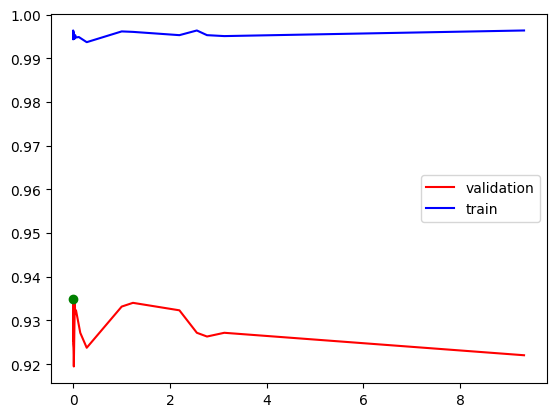
\includegraphics[scale=0.5]{descărcare (1).png}\\
Locating the first template\\
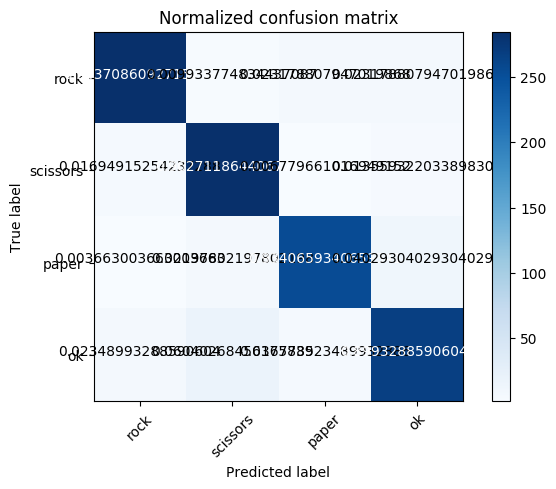
\includegraphics[scale=0.5]{descărcare (2).png}\\
After cutting the first template\\
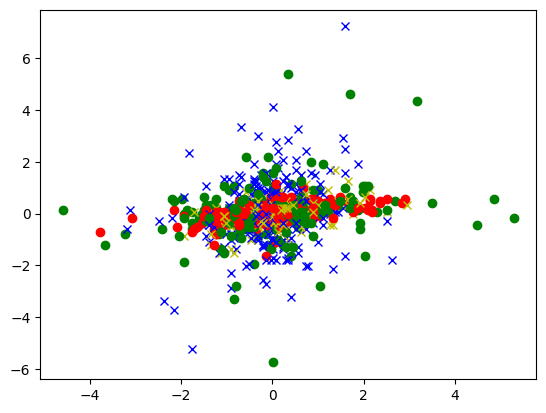
\includegraphics[scale=0.7]{descărcare (3).png}\\
Location of the second template\\
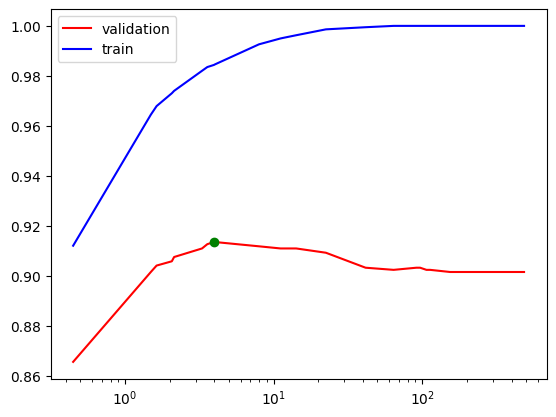
\includegraphics[scale=0.7]{descărcare (4).png}\\
After cutting the second template\\
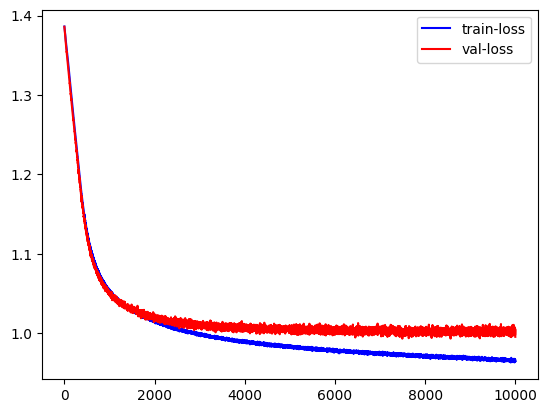
\includegraphics[scale=0.7]{descărcare (5).png}\\
After removing the backround\\
\includegraphics[scale=0.7]{descărcare (6).png}\\
Identification of the first digit\\
\includegraphics[scale=0.7]{descărcare (7).png}\\
Identification of the second digit\\
\includegraphics[scale=0.7]{descărcare (8).png}\\

Where the templates chosen are:

\includegraphics[scale=1]{template_matching.JPG}

\includegraphics[scale=1]{template_matching2.JPG}

\end{document}